\chapter{Resumen del Trabajo Realizado}
Este Trabajo Final de Grado tiene como misión el diseño y desarrollo de una aplicación cuya principal funcionalidad es, la clasificación de  meteoros mediante sonidos generados por ordenador a partir de detecciones de llevadas a cabo mediante radiofrecuencia. 

El proyecto tiene como objetivo ser accesible a personas con discapacidad visual y para ello, se pretende desarrollar una herramienta mediante la cual se pueda seguir una conversación en \textit{lenguaje natural}, estas herramientas se conocen por el término en inglés \textit{chatbot}. Será necesario que la herramienta sea capaz de reconocer la voz y a su vez transmitir mediante voz la información generada por la aplicación.
Esto va a facilitar el acceso a la herramienta no sólo a personas con problemas de visión sino también a niños que aún no sepan leer o escribir.

Por tanto, será necesario realizar un diseño estructural tanto de la base de datos para guardar los distintos parámetros de las radio detecciones, así como de la API que comunique la base de datos con la aplicación y del sitio Web, que deberá tener un diseño \textit{responsive}, es decir, que se adapte a los diferentes dispositivos desde los que se pueda acceder.

Hasta ahora, se ha realizado el diseño y volcado de la base de datos antigua que contenía la información de las radio detecciones, y se ha comenzado la creación de un API Rest para conectar la base de datos con la aplicación.

Además, se han mantenido reuniones semanales entre todos los miembros del proyecto, así como la confección de los documentos intermedios y finales del trabajo.



\chapter{Explicación y justificación de las modificaciones al Plan de Trabajo}

El avance del proyecto se ha visto afectado debido a que depende de personas externas y equipamiento que no está bajo el control de los miembros del equipo.
Para poder realizar el proyecto necesitamos generar sonidos a través de las detecciones de los meteoros.
Hasta ahora los sonidos eran generados mediante varios programas en Python desarrollados por Samuel Lemes Perera para el Citizen Science Lab \cite{Stream Generator} de la Universidad Politécnica de Madrid, aunque el resultado es un sonido bastante artificial y metálico motivo por el cual estamos investigando nuevas formas de generarlos, algo que ha repercutido en la planificación inicial del proyecto.

Debido a estos motivos, la planificación se encuentra en el estado que se desarrolla en los siguientes apartados.
\vspace{1cm}
\section*{Revisión de la lista de objetivos del trabajo}

En lo que llevamos de proyecto se ha diseñado y desarrollado tanto una nueva base de datos como una parte de la API y la documentación de esta. La lista de objetivos sigue siendo la siguiente: 
\begin{itemize}
    \item Mejora de la interfaz conversacional de un chatbot.
    \item Integración de los módulos de reconocimiento y sintetizador de la voz.
    \item Desarrollo de una interfaz web del experimento de clasificación de meteoros para público infantil.
    \item Módulo para analizar los resultados obtenidos.
    \item Desarrollo de una guía de usuario.
\end{itemize}
\vspace{1cm}
\section*{Revisión de la lista de tareas}

Aunque existan ciertos contratiempos y retrasos en el desarrollo del proyecto, la lista de tareas continúa como estaba planificada inicialmente.

\begin{itemize}
    \item T1: Estado del arte de los chatbots. (20 horas).
    \item T2: Análisis de módulos de reconocimiento y sintetizador de voz. (20 horas).
    \item T3: Ampliación del dataset para entrenar el chatbot. (20 horas).
    \item T4: Integración de los módulos de reconocimiento y sintetizador de voz. (50 horas)
    \item T5: Implementación de las mejoras del chatbot (70 horas).
    \item T6: Desarrollo de la interfaz web del experimento. (50 horas).
    \item T7: Despliegue y pruebas con grupos de interés. (44 horas).
    \item T8: Documentación. (50 horas).
\end{itemize}

Total: 324 horas. \textbf{12 ECTS}

Dado que se sigue una metodología \textit{agile} se realiza una reunión un día a la semana de una hora de duración, en la que el equipo cuenta los avances que han realizado y se planifican las siguientes tareas a realizar. Debido a la situación actual, estas reuniones se realizan de forma telemática mediante Skype.

\section*{Revisión del diagrama de Gantt}
De la planificación realizada al inicio del Trabajo de Fin de Grado se creó este diagrama de Gantt. Aunque existan cierto retraso, se mantiene la planificación inicial.

\vspace{0.5cm}
\begin{figure}[h]
    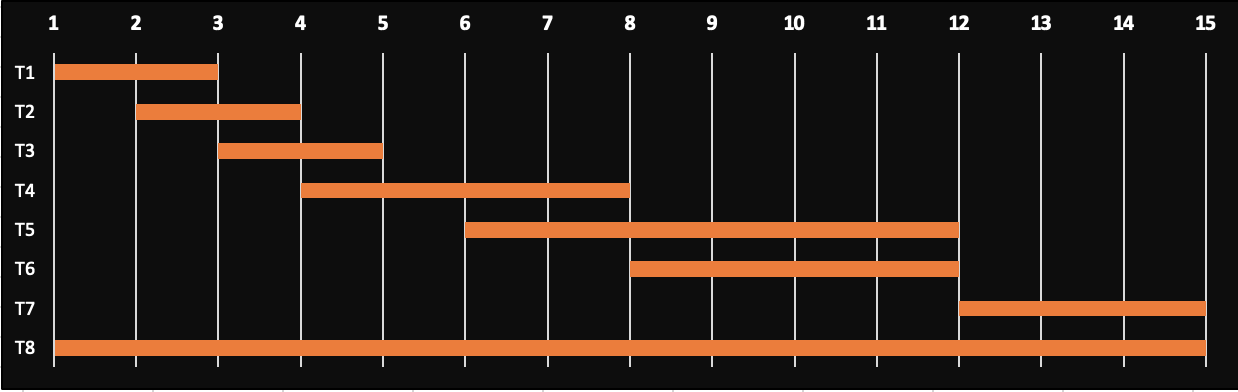
\includegraphics[scale=0.75]{{include/figuras/GanttInicio.png}}
    \caption{Diagrama de Gantt}
    \label{fig:gantt_inicial}
\end{figure}


%%%%%%%%%%%%%%%%%%%%%%%%%%%%%%%%%%%%%%%%%%%%%%%%%%%%%%%%%%%
%% Final del resumen. 
%%%%%%%%%%%%%%%%%%%%%%%%%%%%%%%%%%%%%%%%%%%%%%%%%%%%%%%%%%%